\documentclass[xcolor=svgnames,9pt]{beamer}
\mode<presentation> {\usetheme{Madrid}\setbeamercovered{transparent}}

\usepackage{pstricks}
\usepackage{color}
\usepackage{framed}

\newtheorem{prop}{Proposition}
\newtheorem{thm}{Theorem}[section]
\newtheorem{lem}[thm]{Lemma}

\newtheorem{dfn}{Definition}
\theoremstyle{remark}
\newtheorem*{remark}{Remark}

\definecolor{light-gray}{gray}{0.95}
\setbeamercolor{red1}{fg=black,bg=Bisque}
\setbeamercolor{Lavender}{fg=black,bg=Lavender}
\setbeamercolor{Thistle}{fg=black,bg=Thistle}
\setbeamercolor{Gray}{fg=black,bg=light-gray}

\usefonttheme{professionalfonts}

\title[EQ's effect on multistory buildings]
{\textsc{Earthquake's effect on multistory buildings: a simple model}}

\institute[]{\large \textsc{\v{C}VUT FSv}}

\author[Kalin Ivanov]
{Kalin Ivanov}

\date[15 June 2017]
{Mathematics 2 Semester Project
\\
\bigskip
15 June 2017\\
\bigskip
\bigskip
\bigskip
\small supervised by Ing. Michal Bene\v{s}, Ph.D\par
}

\begin{document}
%TITLE	%%%%%%%%%%%%%%%%%%%%%%%%%%%%%%%%%%%%%%%%%%%%%%%%%%%%%
		\begin{frame}
  			\titlepage
		\end{frame}
%%%%%%%%%%%%%%%%%%%%%%%%%%%%%%%%%%%%%%%%%%%%%%%%%%%%%%%%%%%
	\section{Introduction}
%INTRO	%%%%%%%%%%%%%%%%%%%%%%%%%%%%%%%%%%%%%%%%%%%%%%%%%%%%%
		\begin{frame}
			\frametitle{Model Description}
			\begin{itemize}
				\item Motion of earth caused by earthquake puts buildings into motion
				\item Multistory buildings modelled as point-masses connected via springs and dashpots

				\begin{figure}
 				 	\begin{minipage}[b]{0.4\textwidth}
						\centering
    						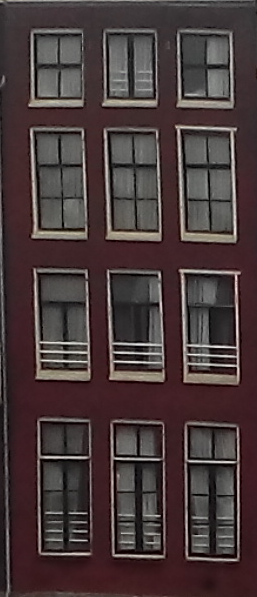
\includegraphics[width=20mm]{bldg.png}
    						\caption{Reality}
						\label{bldg}
  					\end{minipage}
 					 \hfill
					\begin{minipage}[b]{0.4\textwidth}
						\centering
 				  	 	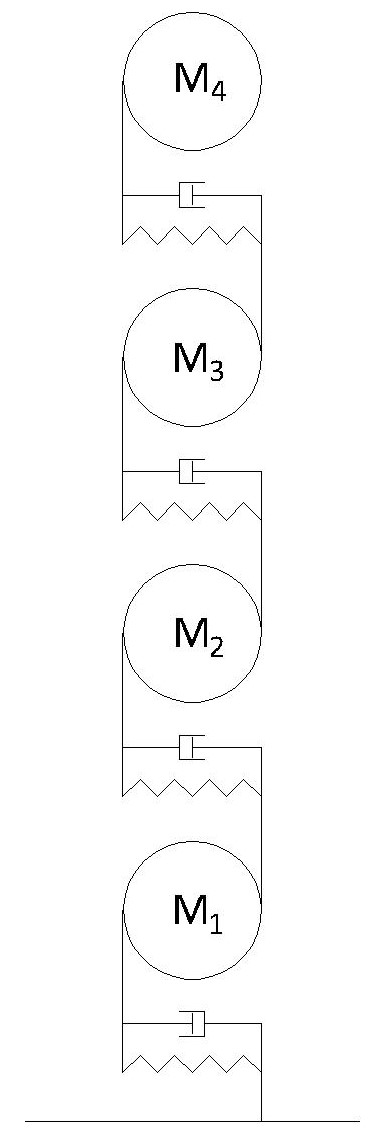
\includegraphics[width=15mm]{SPRINGS-Model1A.jpg}
    						\caption{Simplification}
						\label{Springs1}
 					 \end{minipage}
				\end{figure}

				\item Consider mass $m_i$, spring constant $k_i$, damping constant $c_i$, displacement $x_i$,  and velocity $v_i$ of the $i^{th}$ floor
			\end{itemize}
			\bigskip
		\end{frame}
%PHYSICAL DESCRP	%%%%%%%%%%%%%%%%%%%%%%%%%%%%%%%%%%%%%%%%%%%%%%%
		\begin{frame}
  			\frametitle{Physical Description}
			\begin{itemize}
				\item Forces on each floor depend on the floors above and below
				\begin{figure}
 				 	\begin{minipage}[b]{0.4\textwidth}
						\centering
    						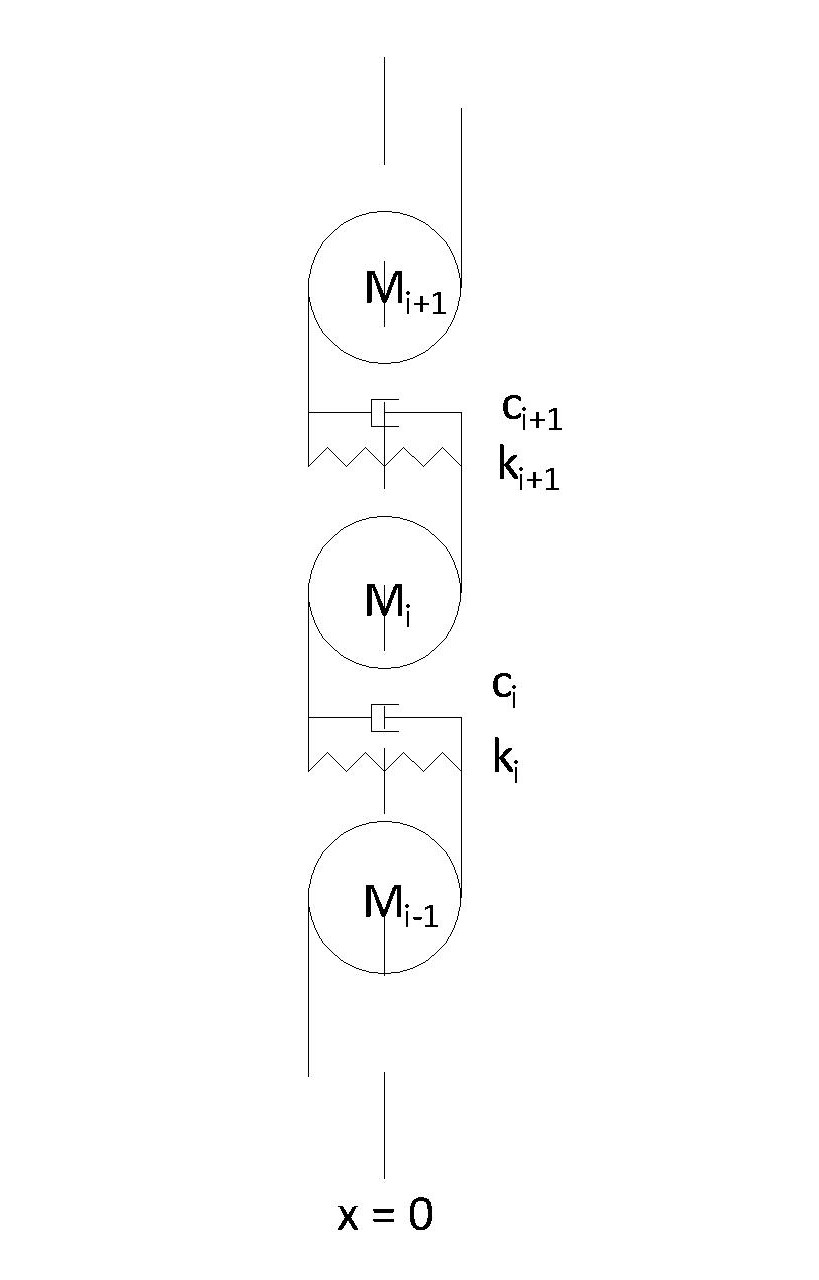
\includegraphics[width=30mm]{SPRINGS-Model2A.jpg}
    						\caption{$i^{th}$ floor statics}
						\label{Springs2}
  					\end{minipage}
 					\hfill
					\begin{minipage}[b]{0.4\textwidth}
						\centering
 				  		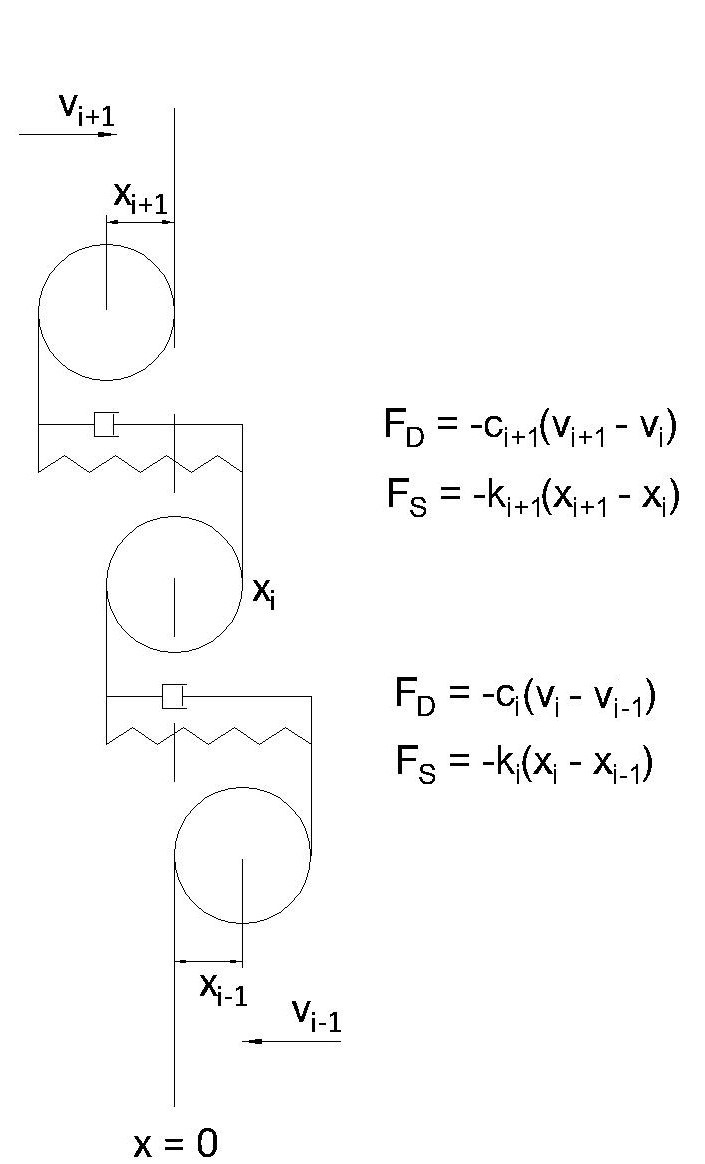
\includegraphics[width=28mm]{SPRINGS-Model3A.jpg}
    						\caption{$i^{th}$ floor dynamics}
						\label{Springs3}
 					\end{minipage}
				\end{figure}
				\item Hooke's law describes the spring force $F_S = - kx$
				\item A linear damping force is considered in a similar manner $F_D = - c\dot{x}$
			\end{itemize}

		\end{frame}
%MOTION EQ	%%%%%%%%%%%%%%%%%%%%%%%%%%%%%%%%%%%%%%%%%%%%%%%%%%
		\begin{frame}
  			\frametitle{Equation of Motion}
			\begin{itemize}
				\item Define system of equations for $n$ floors
			\end{itemize}
				\begin{framed}
					\begin{equation}\label{MotionEQ}
						\textbf{M}\ddot{X}+\textbf{C}\dot{X}+\textbf{K}X = F
					\end{equation}
					\begin{equation*}
						X(0)=D_0 \text{ , }
						\dot{X}(0)=V_0
					\end{equation*}
				\end{framed}
				\begin{equation*}
					\textbf{K}=
					\begin{bmatrix}
						k_1 + k_2 & -k_2 & 0 & 0 & \cdots & 0 & 0 & 0\\
						-k_2 & k_2 + k_3 & -k_3 & 0 & \cdots & 0 & 0 & 0\\
						\vdots & \vdots & \vdots & \vdots & \ddots & \vdots & \vdots & \vdots \\
						0& 0 & 0 & 0 & \cdots & 0 & -k_{n} & k_{n}\\
					\end{bmatrix},\ \ 
				\end{equation*}\\

				\begin{equation*}
					\textbf{C}=
					\begin{bmatrix}
					           c_1 + c_2 & -c_2 & 0 & 0 & \cdots & 0 & 0 & 0\\
						-c_2 &  c_2 + c_3 & -c_3 & 0 & \cdots & 0 & 0 & 0\\
						\vdots & \vdots & \vdots & \vdots & \ddots & \vdots & \vdots & \vdots \\
						0& 0 & 0 & 0 & \cdots & 0 &-c_{n} & c_{n}\\ 
					\end{bmatrix},\ \ 
				\end{equation*}\\

				\begin{equation*}
					\textbf{M}=
					\begin{bmatrix}
						m_1 & 0 & 0 & \cdots & 0\\
						0 & m_2 & 0 & \cdots & 0\\
						\vdots & \vdots & \vdots & \ddots & \vdots \\
						0 & 0 & 0 & \cdots & m_n
					\end{bmatrix},\ \ 
					F=
					\begin{bmatrix}
						f_1(t)\\
						0\\
						\vdots \\
						0
					\end{bmatrix},\ \
					X=
					\begin{bmatrix}
						x_1(t)\\
						\vdots \\
						x_n(t)
					\end{bmatrix}
				\end{equation*}
		\end{frame}
%NEWMARK		%%%%%%%%%%%%%%%%%%%%%%%%%%%%%%%%%%%%%%%%%%%%%%%%%%
		\begin{frame}
  			\frametitle{Newmark Method}
			\begin{itemize}
				\item Discretization of position and velocity using truncated Taylor series expansions that have defined constants $\beta$ and $\gamma$
				\begin{align*}
					&D_{n+1} = D_{n}+V_{n}\Delta t+\frac{A_{{n}}{\Delta t}^{2}}{2}+2\beta \dot{A}_{n}{\Delta t}^3\\
					&V_{n+1} = V_{n}+A_{n}\Delta t+\gamma \dot{A}_{n} \Delta t^2
				\end{align*}
				\item Definition of derivative approximation
				\begin{equation*}
					\dot{A}_{n} = \frac {A_{{n+1}}-A_{{n}}}{\Delta t}
				\end{equation*}
				\item The Newmark method is defined by the following 3 equations
				\begin{equation}
					\textbf{M}A_{n+1}+\textbf{C}V_{n+1}+\textbf{K}X_{n+1} =F_{n+1}
				\end{equation}

				\begin{equation}
					D_{n+1} = D_{n}+V_{n}\Delta t+\frac{{\Delta t}^{2}}{2}[(1-2\beta)A_n + 2\beta A_{n+1}]
				\end{equation}

				\begin{equation}
					V_{n+1} = V_{n}+\Delta t[(1-\gamma)A_n + \gamma A_{n+1}]
				\end{equation}

			\end{itemize}
		\end{frame}
%NEWMARK IMPL		%%%%%%%%%%%%%%%%%%%%%%%%%%%%%%%%%%%%%%%%%%%%%%%
		\begin{frame}
  			\frametitle{Implementation of Newmark Method}
			\begin{enumerate}
				\item Using initial conditions $D_0$ and $V_0$ calculate $A_0$
					\begin{equation*}
						A_{{0}}= \textbf{M}^{-1} (F_{{0}} -\textbf{C}V_{{0}}-\textbf{K}D_{{0}})
					\end{equation*}
				\item Define constants
					\begin{align*}
						&c_1 = {\frac {1}{{\beta \Delta t}^{2}}}\ \ \ \ \ c_2 =\frac{1}{\beta \Delta t }\ \ \ \ \ c_3 = \frac{1}{2\beta}-1\\
						&c_4 = \frac {\gamma}{\beta \Delta t}\ \ \ \ \ c_5 = 1-{\frac {\gamma}{\beta}}\ \ \ \ \ c_6 = \Delta t \left( 1-{\frac {\gamma}{2\beta}} \right)
					\end{align*}
				\item Define inverted matrix allowing for explicit calculation of $D_{n+1}$
					\begin{equation*}
						\left( {\frac {\textbf{M}}{{\Delta t}^{2}\beta}}+{\frac {\textbf{C}\gamma}{\Delta t\,\beta}}+\textbf{K} \right) D_{{n+1}}=F_{{n+1}}+\textbf{M} \left( {\frac {\widetilde{D}_{{n+1}}}{{\Delta t}^{2}\beta}} \right) -\textbf{C}\left({{\widetilde{V}_{{n+1}}-{\frac {\gamma \widetilde{D}_{{n+1}}}{\Delta t\,\beta}}}}\right)
					\end{equation*}
				\item For each time step calculate $D_{n+1}$, $V_{n+1}$ and $A_{n+1}$
					\begin{align*}
						&\widetilde{A}_{{n+1}}=-c_1D_n+c_2V_n+c_3A_n\\
						&\widetilde{V}_{{n+1}}=c_4D_n+c_5V_n+c_6A_n\\
						&D_{{n+1}}=\textbf{W}[F_{{n+1}}+\textbf{M}\widetilde{A}_{{n+1}}-\textbf{C}\widetilde{V}_{{n+1}}]\\
						&V_{n+1} = c_4D_{n+1}+\widetilde{V}_{{n+1}}\\
						&A_{n+1}= c_1D_{n+1}-\widetilde{A}_{{n+1}}
					\end{align*}
			\end{enumerate}
		\end{frame}
%NEWMARK STAB3	%%%%%%%%%%%%%%%%%%%%%%%%%%%%%%%%%%%%%%%%%%%%%%%%
		\begin{frame}
  			\frametitle{Stability of Undamped Motion}
			\begin{itemize}
				\item Stability condition $\rho \leq 1 \Rightarrow \gamma \geq \frac{1}{2}$ and $(\gamma + \frac{1}{2})^2 - 4\beta \leq \frac{4}{\Omega_i^2}$
				\item Unconditionally stable condition
					\begin{equation}
						\beta \geq \frac{1}{4}\left(\gamma + \frac{1}{2}\right)^2
					\end{equation}
				\item Average constant acceleration method: $\gamma = \frac{1}{2}$ and $\beta = \frac{1}{4}$ 
				\begin{figure}[h!]
   					 \centering
   					 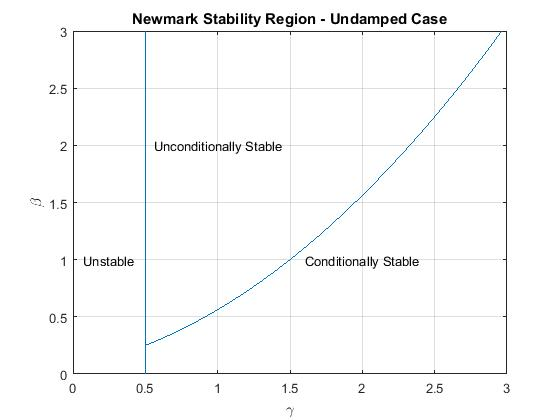
\includegraphics[width=75mm]{GraphNM.jpg}
   					 \caption{Newmark Method Stability Regions}
				            \label{GraphNM}
  				\end{figure}
			\end{itemize}
		\end{frame}
%NEWMARK ACC		%%%%%%%%%%%%%%%%%%%%%%%%%%%%%%%%%%%%%%%%%%%%%%%
		\begin{frame}
  			\frametitle{Accuracy of Newmark Mehthod}
			\begin{itemize}
				\item Consider $\ddot{x} + x = 0$ with initial conditions $x(0) = 1$, $\dot{x}(0) = 0$ and solution  $x = \cos(t)$
				\begin{figure}[h!]
   					 \centering
   					 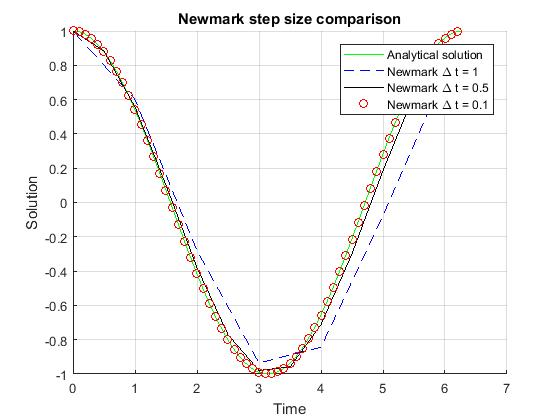
\includegraphics[width=60mm]{NMStepSize.jpg}
   					 \caption{Newmark method solution with different step sizes}
				            \label{fig17}
  				\end{figure}
			\item Amplitude error
\small
				\begin{equation*}
					\rho - 1 = -\frac{1}{2}\left( \gamma - \frac{1}{2} \right)\omega^2\Delta t^2 + O(\Delta t^4)
				\end{equation*}
			\item Periodicity error
				\begin{equation*}
					\frac{\Delta T}{T} =\frac{\omega \Delta t}{\phi} - 1 = \frac{1}{2}\left( \beta - \frac{1}{12} \right)\omega^2\Delta t^2 + O(\Delta t^3)
				\end{equation*}
			\end{itemize}
		\end{frame}
%PARAMS		%%%%%%%%%%%%%%%%%%%%%%%%%%%%%%%%%%%%%%%%%%%%%%%%%%
		\begin{frame}
		\centering
  			\frametitle{Parameters of the Newmark method}
				\begin{tabular}{| l | l | l | l | l | l |}
						\hline & & & & &\\
	Algorithm & $\gamma$ & $\beta$ & $\Omega$ & $\rho -1$ & $\frac{\Delta T}{T}$
						\\ & & & & &
						\\ \hline & & & & &\\
	Unconditionally stable & $1$ & $\frac{3}{2}$ & $\infty$ & $-\frac{\Omega^2}{4}$ & $\frac{17\Omega^2}{24}$
						\\ & & & & &\\
	Conditionally stable & 2 & $\frac{1}{2}$ & 0.97 &$-\frac{3 \Omega^2}{4}$ &  $\frac{5 \Omega^2}{24}$ 
						\\ & & & & &\\
	Unstable & 1 & $\frac{1}{4}$ & 0 & $-\frac{\Omega^2}{4}$ & $\frac{\Omega^2}{12}$ 
						\\ & & & & &\\
	Constant Acceleration & $\frac{1}{2}$ & $\frac{1}{4}$ & $\infty$ & $O(\Delta t^4)$ & $\frac{\Omega^2}{12}$ 
						\\ & & & & &\\
	Purely Explicit & 0 & 0 & 0 & $\frac{\Omega^2}{4}$ & $-\frac{\Omega^2}{24}$
						\\ & & & & &\\
	Linear Acceleration & $\frac{1}{2}$ & $\frac{1}{6}$ & 3.46 & $O(\Delta t^4)$ & $\frac{\Omega^2}{24}$
						\\ & & & & &\\ \hline
    					\end{tabular}
		\end{frame}

%%%%%%%%%%%%%%%%%%%%%%%%%%%%%%%%%%%%%%%%%%%%%%%%%%%%%%%%%%%
\frame{
		\frametitle{Order of Newmark error}
\begin{figure}[h!]
   					 \centering
   					 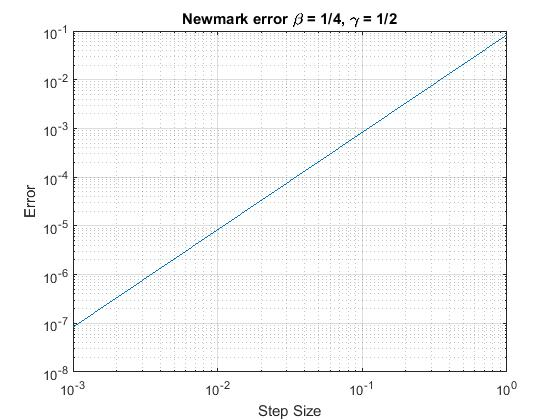
\includegraphics[width=90mm]{error.jpg}
   					 \caption{Newmark method error with different step sizes}
				            \label{fig17}
  				\end{figure}
}
%EL CENTRO	%%%%%%%%%%%%%%%%%%%%%%%%%%%%%%%%%%%%%%%%%%%%%%%%%%
		\begin{frame}
  			\frametitle{El Centro earthquake}
			\begin{itemize}
				\item  Earthquake: 1940, Imperial Valley in California, 6.9 on the Richter Scale
				\item 2-story house: $m_i = 100,000\  kg$, $k_i = 12\text{x}10^5\  \frac{kg}{s^2}$, $c_i = 10^5\ \frac{kg}{s}$
				\begin{figure}[h!]
   					\centering
   					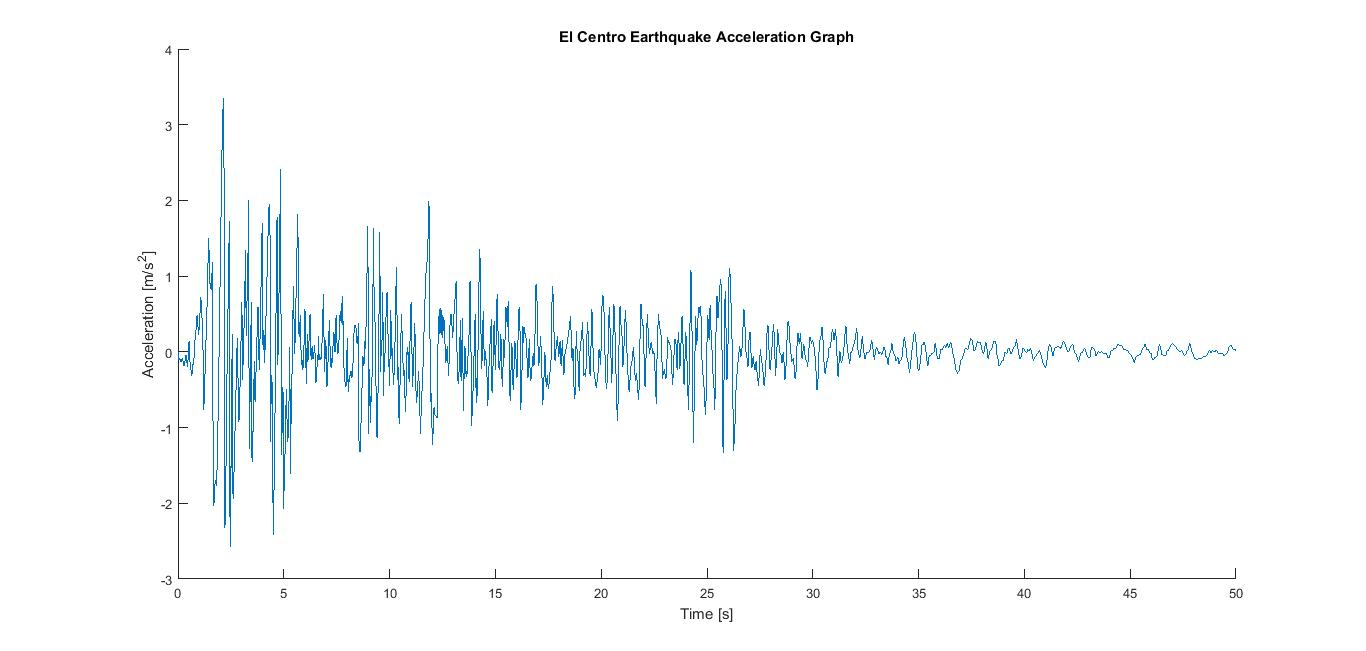
\includegraphics[width=120mm]{ElCentro.jpg}
				           \label{fig10}
					\caption{Acceleration data and 1st floor behavior}
  				\end{figure}
			\end{itemize}
		\end{frame}

%EL CENTRO 2		%%%%%%%%%%%%%%%%%%%%%%%%%%%%%%%%%%%%%%%%%%%%%%%
		\begin{frame}
			\frametitle{El Centro earthquake effect on 2-story house}
				\begin{figure}[h!]
   					\centering
   					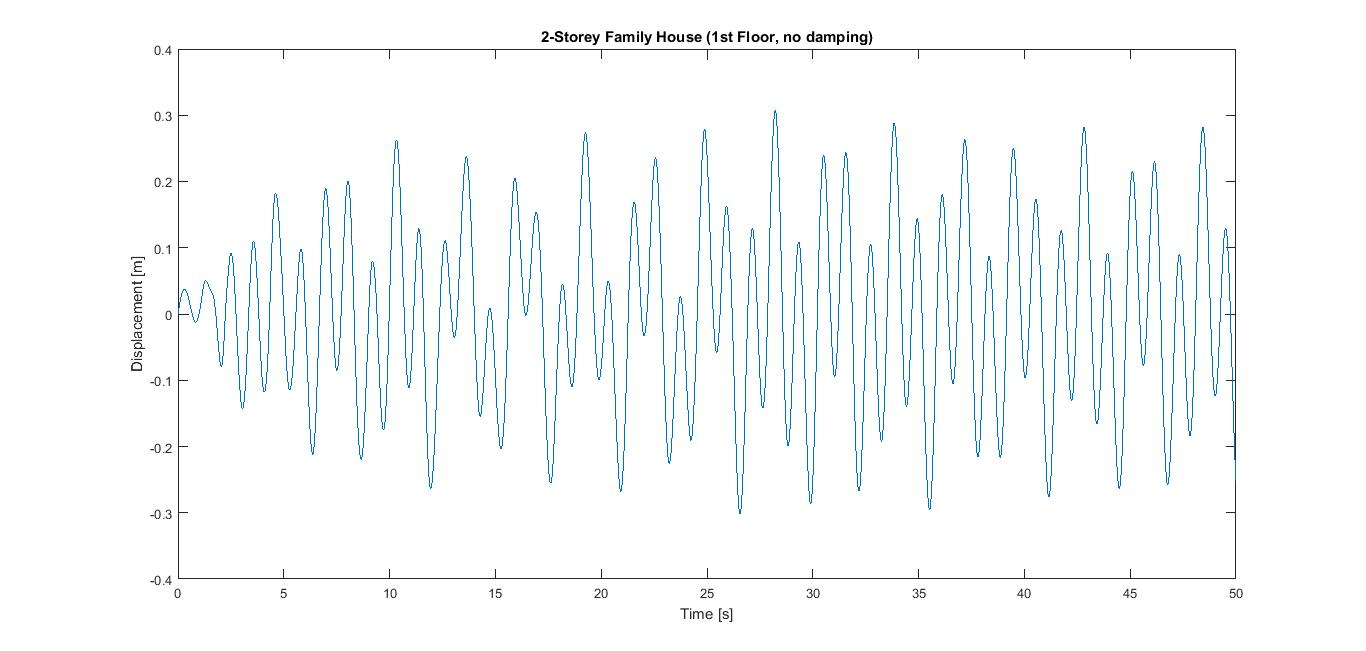
\includegraphics[width=60mm]{FM1.jpg}
					\caption{$1^{st}$ floor without damping}
					\label{FM1}
  				\end{figure}
				\begin{figure}[h!]
   					\centering
   					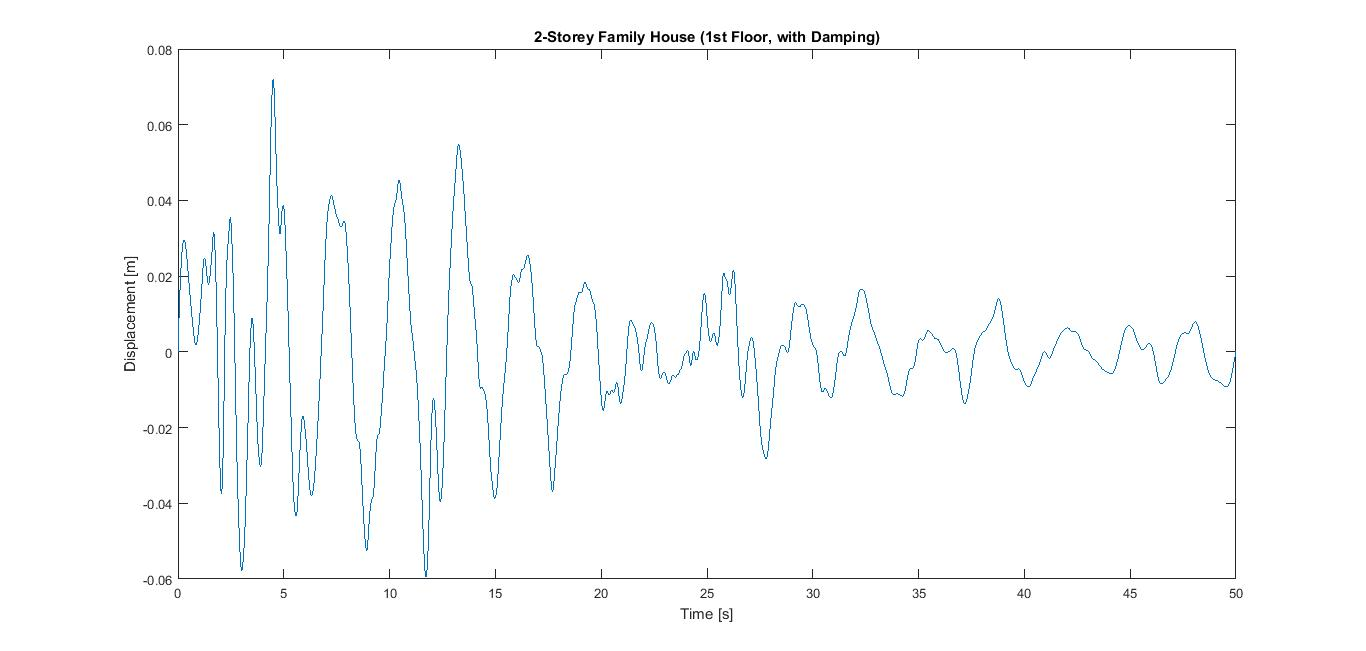
\includegraphics[width=60mm]{FMD1.jpg}
					\caption{$1^{st}$ floor with damping}
					\label{FMD1}
  				\end{figure}
		\end{frame}
%BIBL 	%%%%%%%%%%%%%%%%%%%%%%%%%%%%%%%%%%%%%%%%%%%%%%%%%%%%%
\frame{
\frametitle{Bibliography}

\begin{thebibliography}{9}

\bibitem{A first course in Differential Equations with Modeling Applications} 
Dennis G. Zill
\textit{Differential Equations and Their Applications}. 
Tenth Edition, Loyola Marymount University, Cengage Learning, 2012.

\bibitem{Hughes} 
Thomas J. R. Hughes.
\textit{The Finite Element Method: Linear Static and Dynamic Finite Element Analysis}. 
Chapter 9 Algorithms for Hyperbolic and Parabolic-Hyperbolic Problems, Dover Publications Inc., Mineola, New York, 2000.

\bibitem{Newmark} 
Nathan M. Newmark.
\textit{A Method of Computation for Structural Dynamics}. 
Journal of the Engineering Mechanics Division, Proceedings of the American Society of Civil Engineers, 1959.

\bibitem{Gerardin} 
Michel G\'{e}rardin, Daniel Rixen
\textit{Mechanical Vibrations Theory and Application to Structural Dynamics}. 
Wiley, New York, 1994.

\bibitem{Faustett} 
Laurene V. Fausett
\textit{Applied Numerical Analysis Using MATLAB}. 
Second Edition, Pearson Education Inc., Upper Saddle River, New Jersey, 2008.

\bibitem{Braun} 
Martin Braun
\textit{Differential Equations and Their Applications}. 
Fourth Edition, Springer-Verlag New York Inc., New York, 1993.

\bibitem{IntroToStability} 
Carlos Felippa
\textit{Intoduction to Stability Analysis}. 
Fluid Structure Interaction Chapter 3, University of Colorado at Boulder, 2004.

\bibitem{ElCentro} 
\textit{El Centro Earthquake Page}. 
Vibration Data.

\end{thebibliography}

}
%THANKS		%%%%%%%%%%%%%%%%%%%%%%%%%%%%%%%%%%%%%%%%%%%%%%%%%%%
\frame{

\begin{equation*}
{\huge {\blue \textrm{Thank You For Your Attention!}}}
\end{equation*}

}
%%%%%%%%%%%%%%%%%%%%%%%%%%%%%%%%%%%%%%%%%%%%%%%%%%%%%%%%%%%

\end{document}






